\section{Experimental Results}

\subsection{Implementation}

\begin{figure}[!ht]
\begin{center}
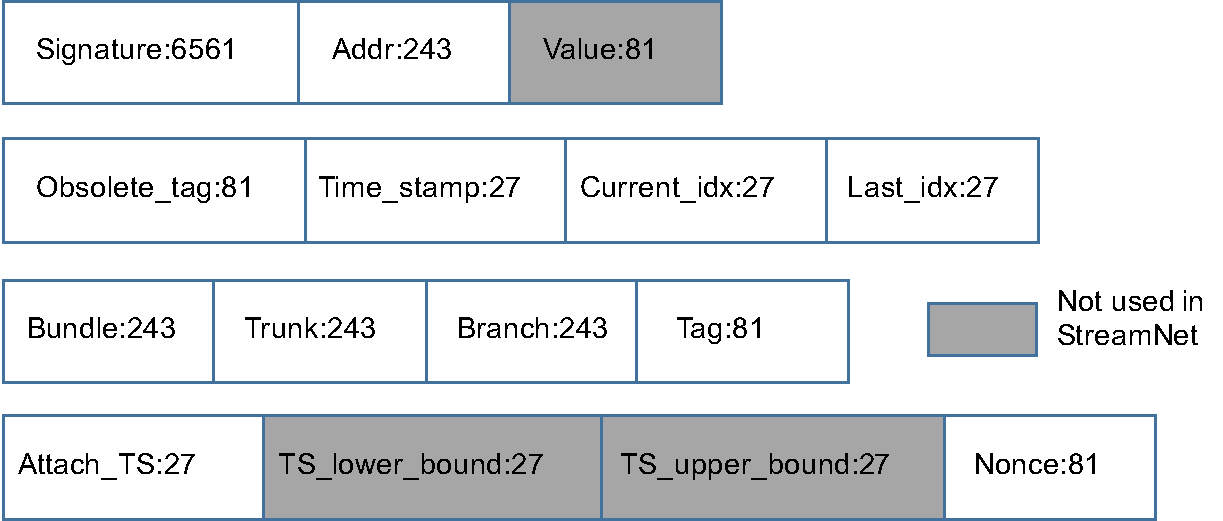
\includegraphics[width=0.45\textwidth]{figures/block_format.pdf}
    \caption{
        Block header format, the main transaction information is stored in the signature part. Addr is sender's address, time stamp is the time the block has been created, current/last index and the bundle are used for storing the bundle information, trunk and branch are the hash address to store the parent and reference location, tag is used for store some tagging information, addtach\_TS is when the block is attached to the StreamNet, nonce is used in POW calculation.
     }
\label{block_header}
\end{center}
\end{figure}

We have implemented the StreamNet based on the IOTA JAVA reference code (IRI) v1.5.5 \cite{IOTACode}.
The code is freely available at \cite{StreamNet}.

\begin{itemize}
    \item The features we have adopted from the IRI are: 
    \begin{itemize}
        \item The block header format, as shown in Figure~\ref{block_header}. Some of the data segments are not used in StreamNet which are marked grey.
        \item Gossip network, the network is a bi-directional network in which every node will send and receive data from its peers;
        \item Trasnaction bundle, because of the existence of the bundle hash feature, StreamNet can support both the single transaction for a block and batched transactions as a bundle. 
        \item Sponge hash functions which is claimed to be quantum immune, in our experiment, the POW hardness is set to 8 which is the same as the testnet for IOTA.
    \end{itemize}

    \item The features we have abandoned from the IRI are:
    \begin{itemize}
        \item The iota's transaction logic inlcuding the ledger validation part;
        \item The milestone issued by coordinators, which is a centralized set up. 
    \end{itemize}

    \item The features we have modified based on the IRI is: 
    \begin{itemize}
        \item The tip selection method based on MCMC, since the tip selection on IRI has to find a milestone to start searching, we replace this with a block in the pivotal chain instead.
    \end{itemize}


    \item The features we have added into the StreamNet are: 
    \begin{itemize}
        \item The consensus algorithms, and we have applied the streaming method directly in the algorithms; 
        \item The UTXO logic which is stored in the signature part of the block header, we used the graph data structure to store UTXO as well. 
        \item In IOTA's implementation, the blocks are stored in the RocksDB \cite{RocksDB} as the persistence layer, which makes it inefficient to infer the relationships between blocks and calculate graph features. In our implementation, we introduced an in-memory layer to store the relationships between blocks, such that the tip selection and total ordering algorithm will be accelerated. 
    \end{itemize}
\end{itemize}

\subsection {Environment Set Up}

\begin{figure*}[!ht]
\begin{center}
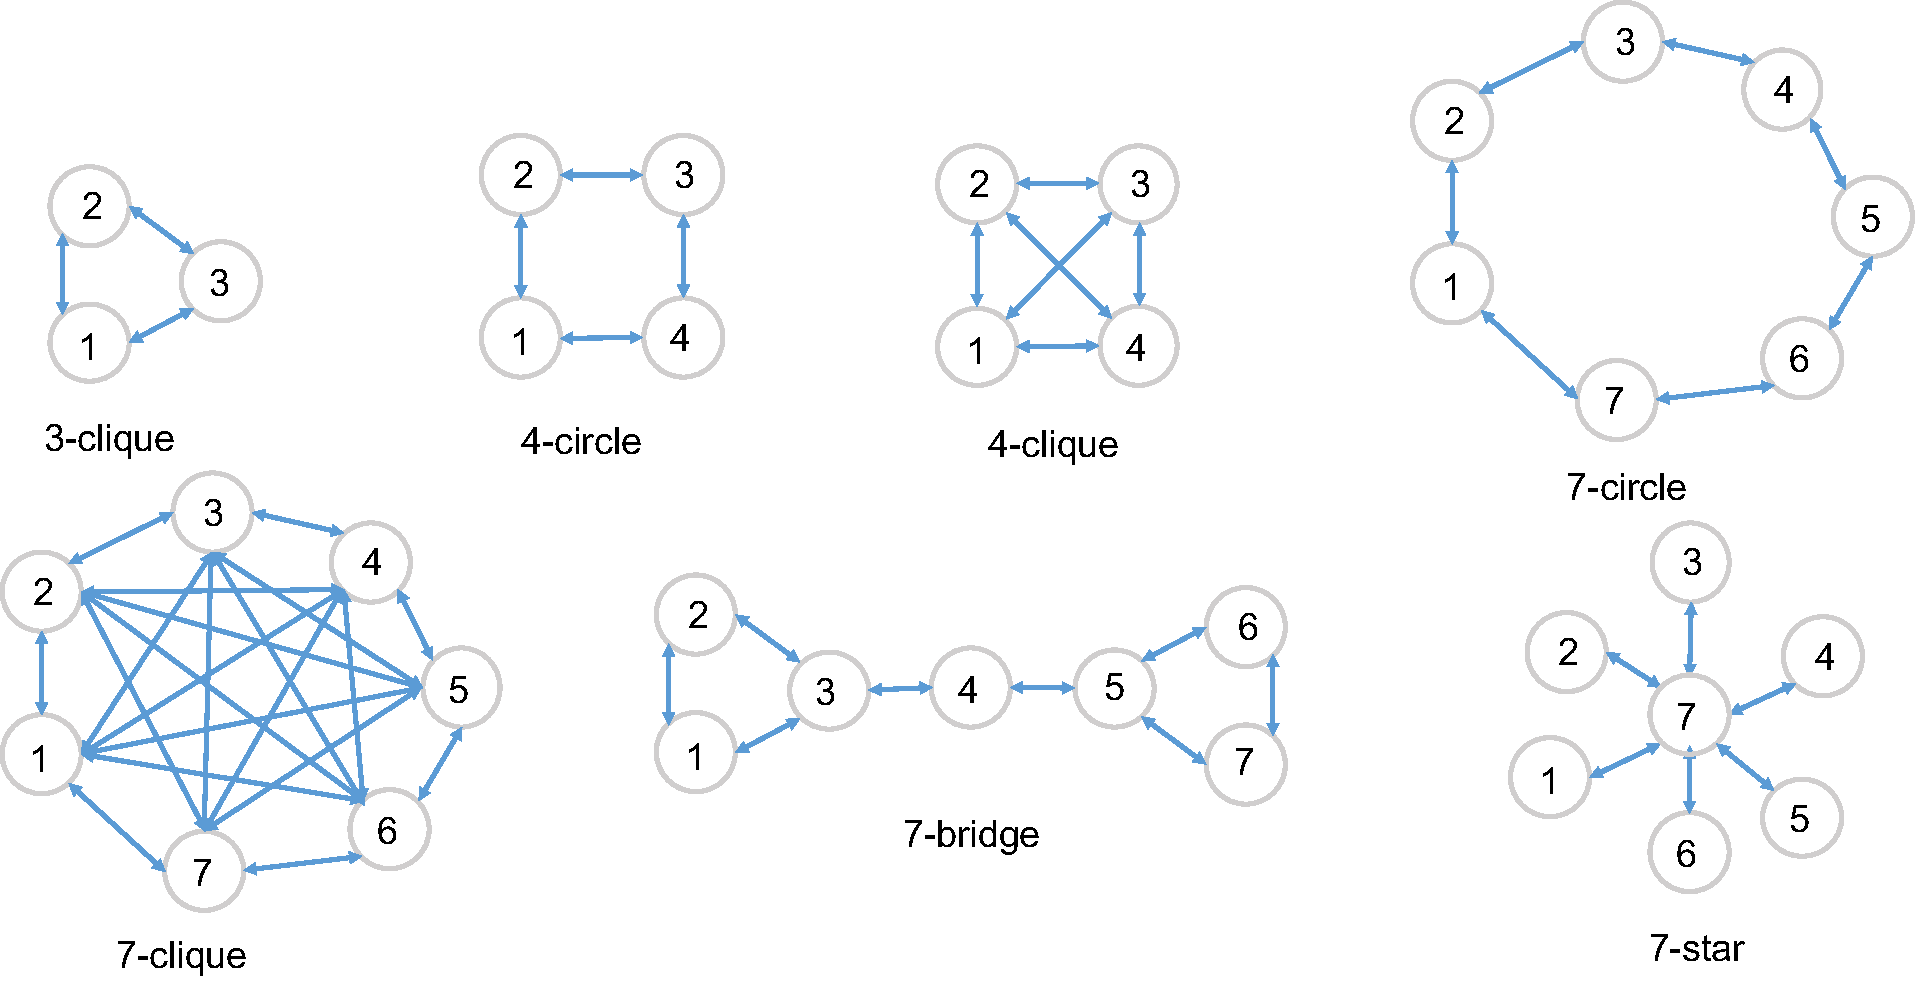
\includegraphics[width=0.75\textwidth]{figures/cluster_set_up.pdf}
    \caption{
        Experimental results for single transaction.
     }
\label{cluster_set_up}
\end{center}
\end{figure*}

We have used the tencent cloud services, for each virtual machine, it includes a two core Intel(R) Xeon(R) CPU E5-26xx v4, with 3 Gb of memory size and 118Gb of disk size. The JAVA version is 1.8, we have deployed our service using docker and the docker version is 18.02.0-ce.   

We have 7 topologies set up of nodes, which are shown in Figure~\ref{cluster_set_up}, these configurations are aiming to test: 
\begin{itemize}
    \item The performance when the cluster connectivity is high (congestion of communications, like 3-clique, 4-clique, 7-clique and 7-star);
    \item The performance when the cluster diameter is high (long hops to pass message, like 4-circle, 7-circle, 7-bridge);
\end{itemize}

As for the data, we have created 10,000 accounts, with the genesis account having 100,000,000,000 tokens in the coinbase block.
And we have issued 1,000,000 transactions in the network with 100 threads.
Jmeter is utilized as the driver to issue the transactions and nginx is used to evenly and randomly distribute the requests to different nodes.

\subsection {Results and Discussions}

\subsubsection {Single transaction test}
By default, each block in StreamNet will only support one transaction. And the performance on this configuration is as Figure~\ref{single_txn} shows.

\begin{figure}[!ht]
\begin{center}
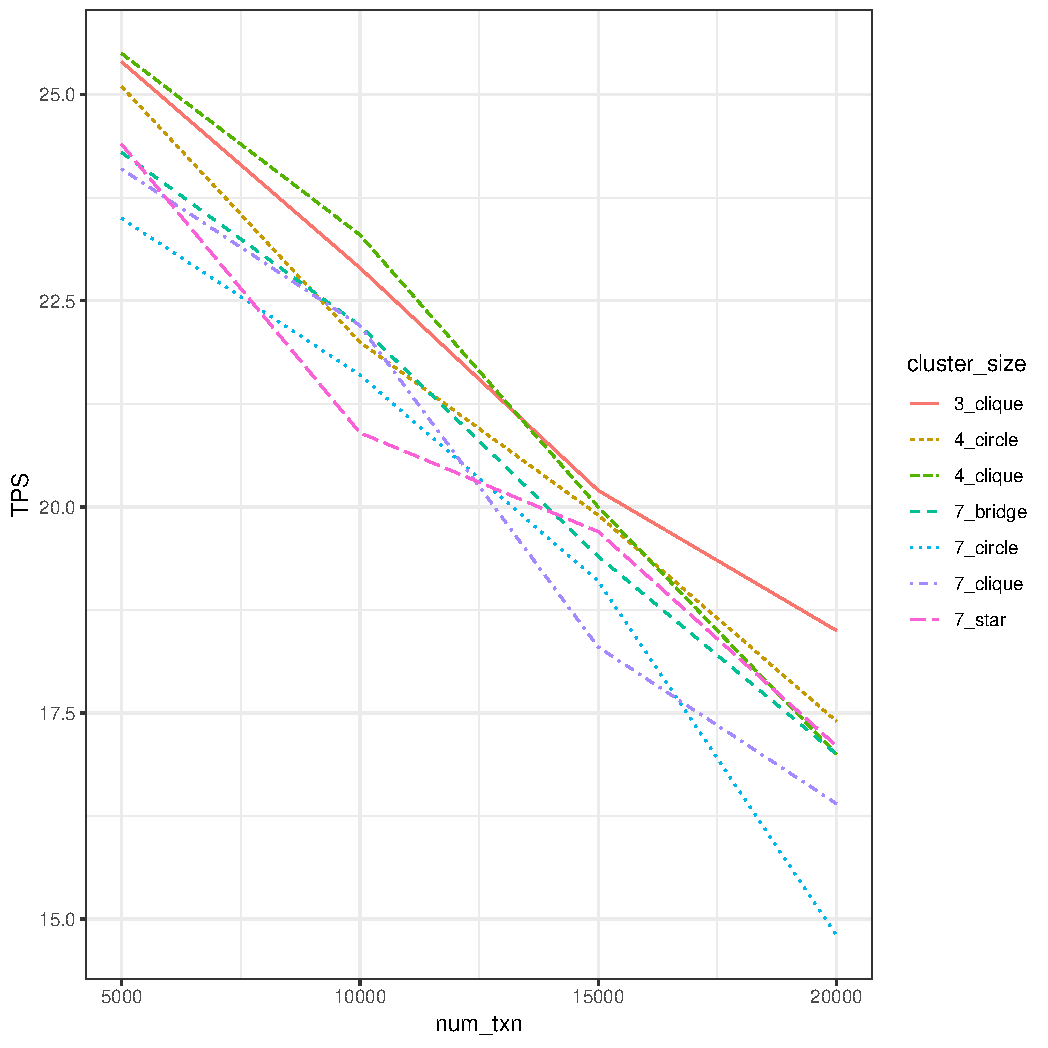
\includegraphics[width=0.45\textwidth]{figures/single_txn.pdf}
    \caption{
        Experimental results for single transaction.
     }
\label{single_txn}
\end{center}
\end{figure}



\subsubsection {Bundle transaction test}

By default, each block in StreamNet will only support one transaction. And the performance on this configuration is as Figure~\ref{multi_txn} shows.

\begin{figure}[!ht]
\begin{center}
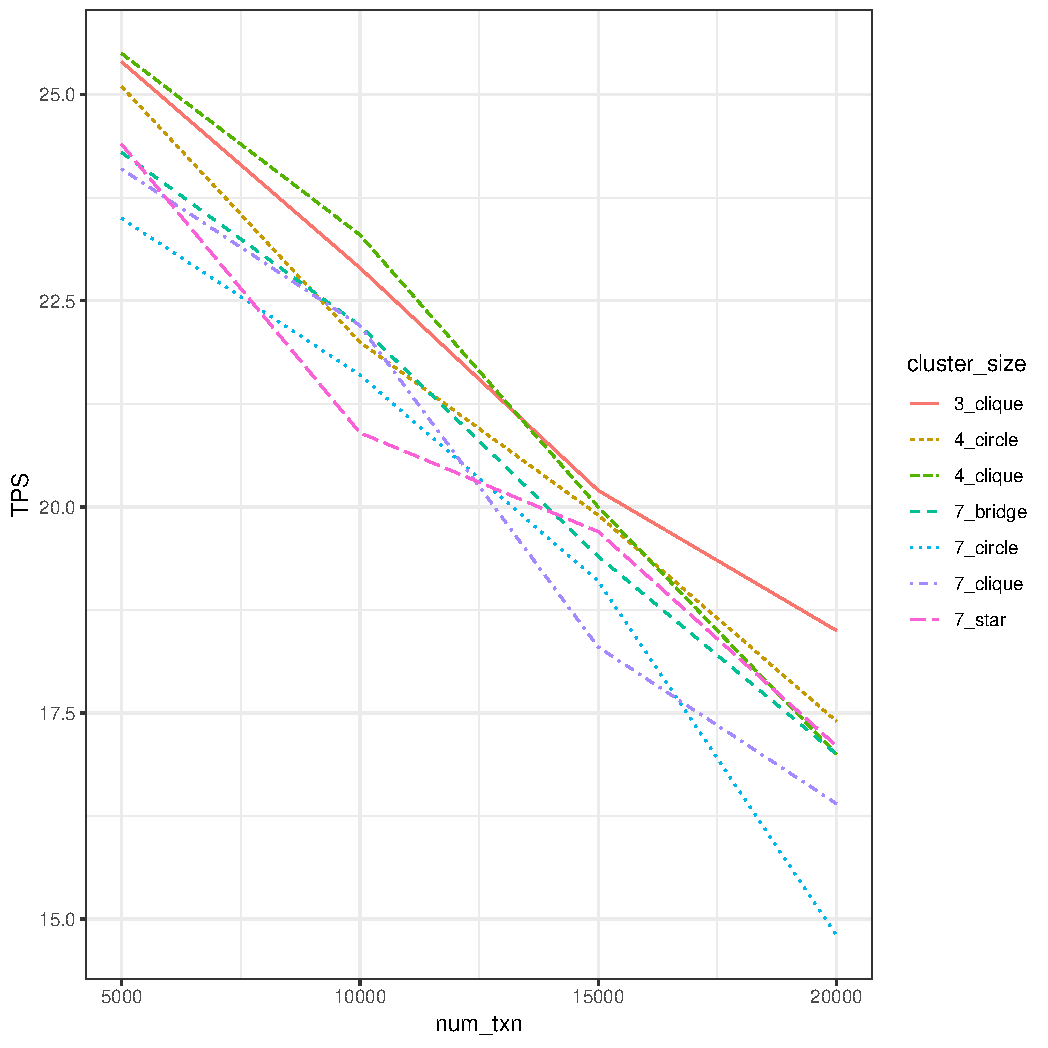
\includegraphics[width=0.45\textwidth]{figures/single_txn.pdf}
    \caption{
        Experimental results for single transaction.
     }
\label{multi_txn}
\end{center}
\end{figure}


